\documentclass[british]{etsbook}
%% \usepackage{otminionpro}                % and otminionmath, if you want
\usepackage{tikz}                          % for the coverfigure
\usepackage{lipsum}                        % for blindtexts
\usepackage{hyperref}                      % no other package here loads it
\usepackage[noabbrev,nameinlink]{cleveref} % for the \cref at the end.
\setmainfont{EBGaramond}  % alternatively, use the otminionpro package

\begin{document}

\title      {Typesetting books}
\author     {Emil Bunsenbrenner}
\subject    {Lecture Notes}
\publishers {University of \LaTeX}
\date       {Summer term 2025}
\coverfigure{%% A neat collection of circles.  This requires the tikz package.
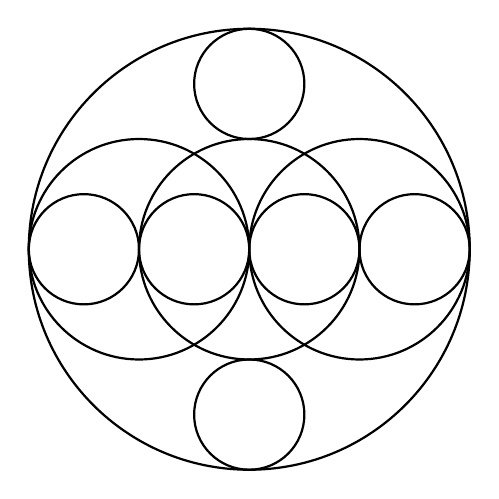
\begin{tikzpicture}[scale=.7]
  \tikzset{every path/.style={thick}}
  \draw ( 0, 0) circle (4);
  \draw ( 0, 0) circle (2);
  \draw ( 2, 0) circle (2);
  \draw (-2, 0) circle (2);
  \draw ( 1, 0) circle (1);
  \draw ( 3, 0) circle (1);
  \draw (-1, 0) circle (1);
  \draw (-3, 0) circle (1);
  \draw ( 0, 3) circle (1);
  \draw ( 0,-3) circle (1);
\end{tikzpicture}
}

\maketitle

\chapter*{Foreword}
\lipsum[1-3]

\tableofcontents{}

%% The upcoming chapter/section/subsection names are copied from Bringhurst’s
%% book (and adapted to British English).

\chapter{The Grand Design}

\section{First principles}

\subsection{Typography exists to honour content.}
\lipsum[4-8]

\subsection{Letters have a life and dignity of their own.}
\lipsum[8-11]

\subsection{There is a style beyond style.}
\lipsum[12-15]

\section{Tactics}
\lipsum[16]

\chapter{Rhythm \emph{\&} Proportion}
\lipsum[1-2]

\section{Horizontal Motion}
\lipsum[3-5]

\section{Footnotes and Sidenotes}

Here you can see a footnote\footnote{\lipsum[1][1-3]}, another
one\footnote{\lipsum[1][4-5]}, and a side note.\marginline{\small
  \lipsum[1][5-7]} \lipsum[2-5]

\section[Webdesign with \acr{CSS}]{Webdesign with CSS}

This is how I would use acronyms in section titles, in order to avoid a clash of
tracking contexts.  Finally, a reference to \cref{fig:circles}.

\begin{figure}
  \centering
  %% A neat collection of circles.  This requires the tikz package.
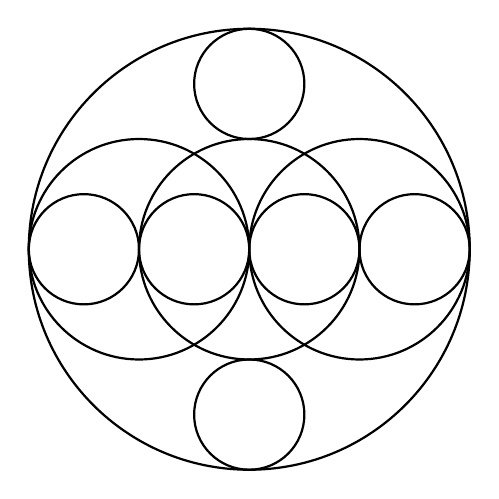
\begin{tikzpicture}[scale=.7]
  \tikzset{every path/.style={thick}}
  \draw ( 0, 0) circle (4);
  \draw ( 0, 0) circle (2);
  \draw ( 2, 0) circle (2);
  \draw (-2, 0) circle (2);
  \draw ( 1, 0) circle (1);
  \draw ( 3, 0) circle (1);
  \draw (-1, 0) circle (1);
  \draw (-3, 0) circle (1);
  \draw ( 0, 3) circle (1);
  \draw ( 0,-3) circle (1);
\end{tikzpicture}

  \caption{A collection of circles. \lipsum[1][1-3]}\label{fig:circles}
\end{figure}

\end{document}



